% ------------------------------------------------------------------------------
% TYPO3 CMS 7.5 - What's New - Chapter "Introduction" (Russian Version)
%
% @author	Michael Schams <schams.net>
% @license	Creative Commons BY-NC-SA 3.0
% @link		http://typo3.org/download/release-notes/whats-new/
% @language	Russian
% ------------------------------------------------------------------------------
% LTXE-CHAPTER-UID:		3a84d600-9fb67dda-31c4af65-dd7a4af5
% LTXE-CHAPTER-NAME:	Introduction
% ------------------------------------------------------------------------------

\section{Введение}
\begin{frame}[fragile]
	\frametitle{Введение}

	\begin{center}\huge{Введение}\end{center}
	\begin{center}\huge{\color{typo3darkgrey}\textbf{Факты}}\end{center}

\end{frame}

% ------------------------------------------------------------------------------
% LTXE-SLIDE-START
% LTXE-SLIDE-UID:		2cc07dc2-a0a38cdb-e07cefe3-d2807266
% LTXE-SLIDE-ORIGIN:	81d53787-fb3806f0-841b4042-7033fad4 English
% LTXE-SLIDE-ORIGIN:	f1ea1041-2b6b2b81-f54b45c0-84265d6a German
% LTXE-SLIDE-TITLE:		TYPO3 CMS 7.5 - The Facts
% ------------------------------------------------------------------------------
\begin{frame}[fragile]
	\frametitle{Введение}
	\framesubtitle{TYPO3 CMS 7.5 - факты}

	\begin{itemize}
		\item Release date: 29. September 2015
		\item Тип: "Sprint Release"
		\item Направленность: охват, инновации, доступность
		\item Primary focus: Finalization
	\end{itemize}

	\begin{figure}
		
\includegraphics[width=0.95\linewidth]{Introduction/typo3cms75-banner.jpg}
	\end{figure}

\end{frame}

% ------------------------------------------------------------------------------
% LTXE-SLIDE-START
% LTXE-SLIDE-UID:		4790a6ef-3b437351-72185642-c5b5fc10
% LTXE-SLIDE-ORIGIN:	a0327db8-b4a9bd42-f32515d0-87296684 English
% LTXE-SLIDE-ORIGIN:	5d8adc7d-af29cb46-4acd2255-27362935 German
% LTXE-SLIDE-TITLE:		System Requirements
% ------------------------------------------------------------------------------
\begin{frame}[fragile]
	\frametitle{Введение}
	\framesubtitle{Системные требования}

	\begin{itemize}
		\item PHP*:\tabto{4cm}v5.5.0 - v5.6.x
		\item MySQL:\tabto{4cm}v5.5.x - v5.6.x (no strict mode)
		\item Дисковое пространство:\tabto{4cm}мин. 200 МБ
		\item PHP настройки:

			\begin{itemize}
				\item memory\_limit >= 128M
				\item max\_execution\_time >= 240s
				\item параметр компиляции \texttt{--disable-ipv6} \underline{не} должен использоваться
			\end{itemize}

		\item Внутренний интерфейс требует IE >= 9 или любой другой современный браузер

	\end{itemize}

	\vspace{1cm}

	*) Подробности: \href{http://typo3.org/news/article/php-minimum-requirements-for-typo3-cms-7/}{PHP Minimum Requirements for TYPO3 CMS 7}

\end{frame}

% ------------------------------------------------------------------------------
% LTXE-SLIDE-START
% LTXE-SLIDE-UID:		17e66114-bdf2265c-547cf4ba-32a1a46a
% LTXE-SLIDE-ORIGIN:	c155d534-1a53682d-f56423dc-163111d3 English
% LTXE-SLIDE-ORIGIN:	6cad14bf-08874e74-1dd85333-e5c43a08 German
% LTXE-SLIDE-TITLE:		Development And Release Timeline
% ------------------------------------------------------------------------------
\begin{frame}[fragile]
	\frametitle{Введение}
	\framesubtitle{График разработки и выхода}

	\begin{figure}
		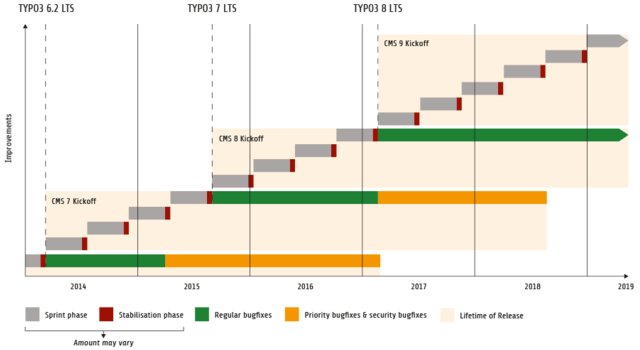
\includegraphics[width=0.90\linewidth]{Introduction/ReleaseAgenda.png}
	\end{figure}

\end{frame}

% ------------------------------------------------------------------------------
% LTXE-SLIDE-START
% LTXE-SLIDE-UID:		10a1aaba-32c6229f-959b22b6-f8a6e628
% LTXE-SLIDE-ORIGIN:	83c1fb1c-ed592fa9-a2a279bd-be5cc800 English
% LTXE-SLIDE-ORIGIN:	387f7aeb-53ab533f-95427547-3aa76412 German
% LTXE-SLIDE-TITLE:		TYPO3 CMS Roadmap
% ------------------------------------------------------------------------------
\begin{frame}[fragile]
	\frametitle{Введение}
	\framesubtitle{Маршрутная карта TYPO3 CMS}

	Примерные даты выхода и их направленность:

	\begin{itemize}
		\item v7.0 \tabto{1.1cm}02/Dec/2014\tabto{3.4cm}Переработка внутреннего интерфейса часть 1
		\item v7.1 \tabto{1.1cm}24/Feb/2015\tabto{3.4cm}Чистка ядра и оптимизация
		\item v7.2 \tabto{1.1cm}28/Apr/2015\tabto{3.4cm}Внешний интерфейс
		\item v7.3 \tabto{1.1cm}16/Jun/2015\tabto{3.4cm}Экосистема пакетов, Composer\newline
			\tabto{3.4cm}и работа с расширениями
		\item v7.4 \tabto{1.1cm}04/Aug/2015\tabto{3.4cm}Переработка внутреннего интерфейса часть 2

		\item
			\begingroup
				\color{typo3orange}
					v7.5 \tabto{1.1cm}29/Sep/2015\tabto{3.4cm}Finalization
			\endgroup

		\item v7 LTS \tabto{1.1cm}Oct/Nov/2015\tabto{3.4cm}\textbf{TYPO3 CMS 7 LTS} (Long Term Release)
	\end{itemize}

	\smaller
		\url{https://typo3.org/typo3-cms/roadmap/}\newline
		\url{http://typo3.org/news/article/embrace-and-innovate-typo3-cms-7/}
	\normalsize

\end{frame}

% ------------------------------------------------------------------------------
% LTXE-SLIDE-START
% LTXE-SLIDE-UID:		78f16d1f-7108e1f6-adf9a807-8ace02e3
% LTXE-SLIDE-ORIGIN:	63decc15-57478e30-70c7ae99-27abd3c2 English
% LTXE-SLIDE-ORIGIN:	3b01edfd-6f06e241-2670b2ad-1b598b4e German
% LTXE-SLIDE-TITLE:		Installation
% ------------------------------------------------------------------------------
\begin{frame}[fragile]
	\frametitle{Введение}
	\framesubtitle{Установка}

	\begin{itemize}
		\item Официальная процедура установки под Linux/Mac OS X\newline
			(DocumentRoot, например \texttt{/var/www/site/htdocs}):
		\begin{lstlisting}
			$ cd /var/www/site
			$ wget --content-disposition get.typo3.org/7.5
			$ tar xzf typo3_src-7.5.0.tar.gz
			$ cd htdocs
			$ ln -s ../typo3_src-7.5.0 typo3_src
			$ ln -s typo3_src/index.php
			$ ln -s typo3_src/typo3
			$ touch FIRST_INSTALL
		\end{lstlisting}

		\item Symbolic links под Microsoft Windows:

			\begin{itemize}
				\item Используйте \texttt{junction} под Windows XP/2000
				\item Используйте \texttt{mmlink} под Windows Vista и Windows 7
			\end{itemize}

	\end{itemize}
\end{frame}

% ------------------------------------------------------------------------------
% LTXE-SLIDE-START
% LTXE-SLIDE-UID:		c21d4872-19a76ddf-d628aa19-40227661
% LTXE-SLIDE-ORIGIN:	4dbfb1f2-70930473-ec804474-1c2ac93a English
% LTXE-SLIDE-ORIGIN:	22ce445c-fe028a61-d11c8f8c-510270d3 German
% LTXE-SLIDE-TITLE:		Upgrade to TYPO3 CMS 7
% ------------------------------------------------------------------------------
\begin{frame}[fragile]
	\frametitle{Введение}
	\framesubtitle{Обновление до TYPO3 CMS 7.x}

	\begin{itemize}
		\item Обновление возможно лишь с TYPO3 CMS 6.2 LTS
		\item Сначала TYPO3 CMS < 6.2 необходимо обновить до TYPO3 CMS 6.2 LTS
	\end{itemize}

	\begin{itemize}

		\item Инструкции по обновлению:\newline
			\smaller\url{http://wiki.typo3.org/Upgrade#Upgrading_to_7.3}\normalsize
		\item Официальное руководство TYPO3 "TYPO3 Installation and Upgrading":
			\smaller\url{http://docs.typo3.org/typo3cms/InstallationGuide}\normalsize
		\item Общий подход:
			\begin{itemize}
				\item \smaller Проверка минимальных системных требований \small(PHP, MySQL и т. д.)
				\item \smaller Просмотр \textbf{deprecation\_*.log} из старой установки TYPO3
				\item \smaller Обновление всех расширений до последних версий
				\item \smaller Загрузка новых исходных файлов и запуск Install Tool \textrightarrow Upgrade Wizard
				\item \smaller Обзор модулей, запускаемых для внутренних пользователей (не обязательно)
			\end{itemize}
	\end{itemize}

\end{frame}

% ------------------------------------------------------------------------------
